\chapter{Introdução}

Dendrímeros são macromoléculas sintéticas também conhecidas como uma espécie de polímeros altamente ramificados \cite{Vogtle2000}.
Eles são estruturados com base em três blocos de construção: o bloco nuclear, o intermediário e o terminal.
Sua organização se dá em camadas de blocos intermediários que crescem a partir do núcleo até a última camada com blocos terminais, como ilustrado na Figura \ref{PAMAMPPI}.
Para cada camada de unidades intermediárias que são adicionadas, dizemos que a geração do dendrímero aumentou em uma unidade.
O número da geração é comumente utilizado como um indicativo do tamanho da molécula\cite{Tomalia1990}.
Nesse trabalho, os dendrímeros serão tratados pelo seu nome seguido da geração, por exemplo, PAMAMG3 para o Poli(amido amina) (PAMAM) de terceira geração com núcleo de etileno diamina (EDA) e PPIG4 para o Poli(propileno imina) (PPI) de quarta geração com núcleo de 1,4-diamino butano (DAB), ilustrados na Figura \ref{PAMAMPPI}.
Ou seja, $GN$ é o identificador do dendrímero de geração $N$.
Sua síntese controlada foi primeiramente proposta por Vögtle \textit{et al}\cite{Vogtle1978} em 1978, mas somente em 1990 que Tomalia \textit{et al}\cite{Tomalia1990} explorou as potenciais aplicações para a estrutura.


\begin{figure}[ht!]
\centering
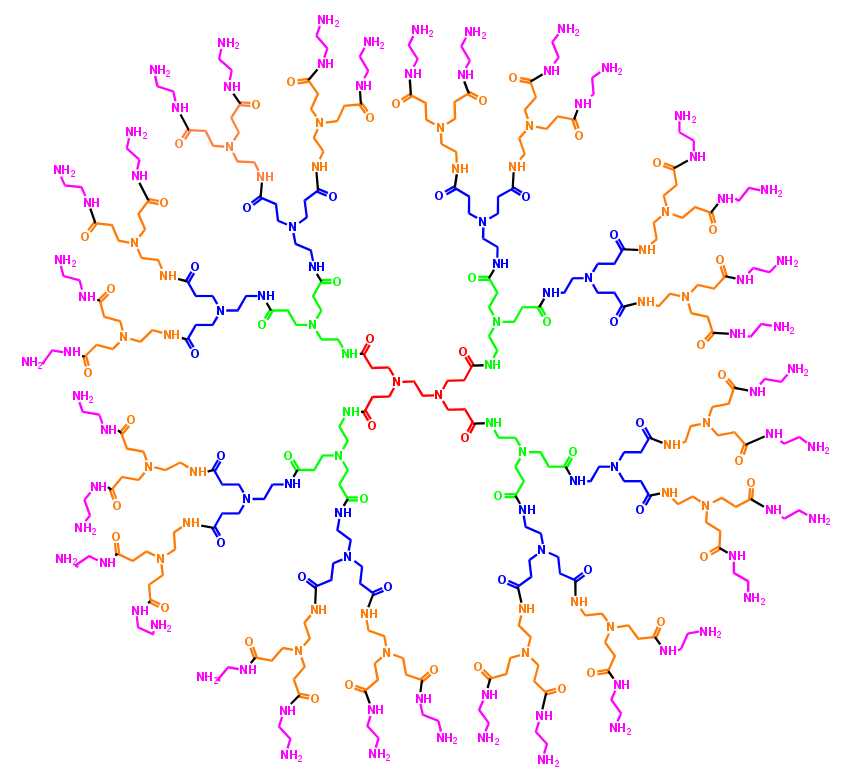
\includegraphics[width=0.45\textwidth]{PAMAM.png}
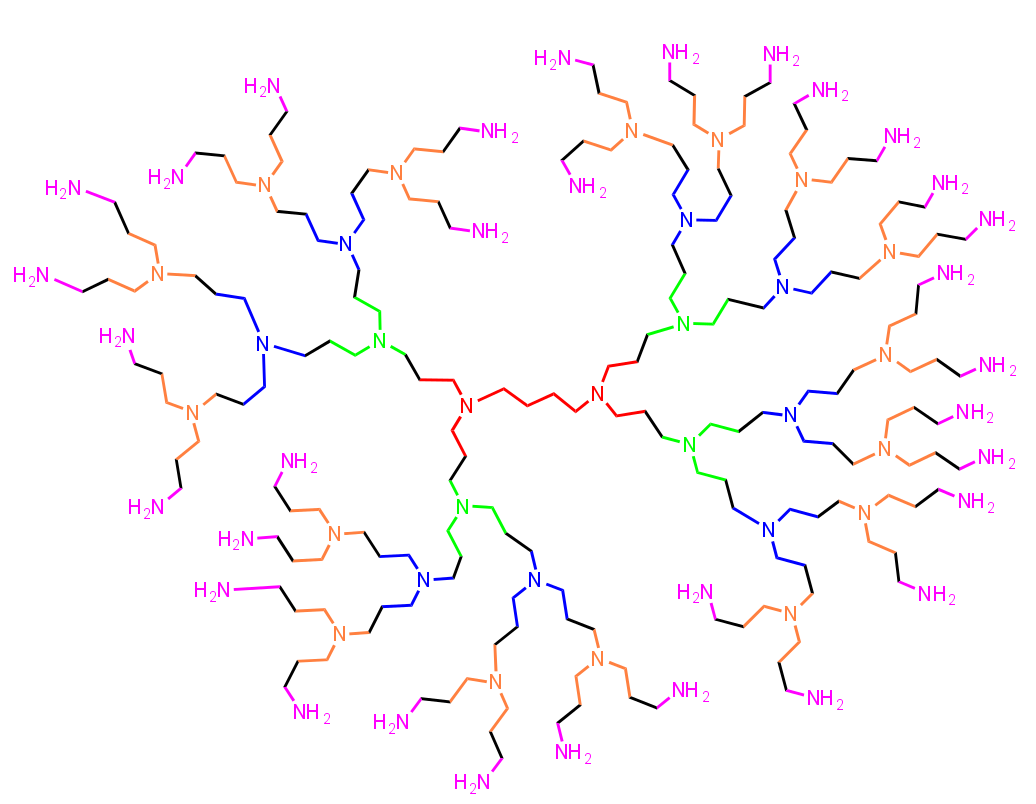
\includegraphics[width=0.45\textwidth]{PPI.png}
\caption{Estrutura química dos dendrímeros Poli(amido amina) (PAMAM) de geração três com núcleo de etileno diamina (EDA) à esquerda e Poli(propileno imina) (PPI) de geração quatro com núcleo de 1,4-diamino butano (DAB) à direita. As cores mostram a camada de blocos intermediários pertencentes à mesma geração. Segundo a nomenclatura utilizada para o PAMAM: O bloco nuclear é mostrado em vermelho, a geração um em verde, a segunda geração em azul, a terceira em laranja e, em rosa, os blocos terminais.}
\label{PAMAMPPI}
\end{figure}

A grande variedade de aplicações atribuídas aos dendrímeros se deve à sua forma tridimensional\cite{Vogtle2000}.
Sua estrutura pode ser dividida em três regiões: a superfície, o espaço entre as cadeias ramificadas e o núcleo do dendrímero\cite{Dykes2001}.
Dependendo da estrutura química da molécula, cada uma dessas regiões pode ter um comportamento distinto e expressar um ambiente químico diferente.
Isso tem verificado às estruturas dendrídicas diversas aplicações em:
Sensores\cite{ChristineValerio1997, Balzani2000},
catalisadores\cite{Kainz2014,Deraedt2017, P.Bhyrappa1996},
processos de separação\cite{Song2017, Song2017a},
\textit{light-harvesting}\cite{Gilat1999, Adronov2000, Andrews2012},
produção de materiais\cite{Gaertner2011, Arshadi2017, Xie2005},
entre outras.
Dentre as aplicações dos dendrímeros, uma de especial interesse é no seu uso como carreadores de fármacos em \textit{Drug-Delivery Systems} (DDS)\cite{Li2010, Svenson2005, Wei2015, Wang2018, Yesil-Celiktas2017}.
Cuja principais regiões utilizadas são as regiões entre as cadeias ramificadas para a solubilização dos fármacos e a superfície para funcionalização e melhorias na seletividade da liberação.
As modificações mais comuns encontradas são a adição de cadeias de Poli(etileno glicol) (PEG) e Poli(óxido de etileno) (PEO) nas cadeias terminais do dendrímero para reduzir sua toxicidade\cite{Sousa2018}.

Como os dendrímeros são altamente personalizáveis, estando sua síntese limitada somente pela criatividade do pesquisador que a está desenvolvendo, muitos novos dendrímeros têm sido relatados na literatura e a definição anterior tem sido estendida recentemente.
De fato, muitas das aplicações podem ser melhoradas com funcionalizações das unidade terminais. 
Nesse âmbito, vêm sido publicados na literatura dendrímeros não-simétricos\cite{Wang2018} (como o Janus\cite{Zhang2014, Gao2014, Dengiz2015}, por exemplo), híbridos\cite{Kavyani2016}, e com funcionalizações na superfície\cite{Barraza2017, Sousa2018, Lee2011, Chooi2010}.

O entendimento da estrutura, das propriedades, do comportamento físico-químico e da interação dos dendrímeros com o meio são informações de vital importância para o conhecimento desse tipo de sistemas, para o desenvolvimento de novas tecnologias e para a projeção de melhorias nas já existentes.
Inicialmente o estudo de dendrímeros foi feito majoritariamente por técnicas experimentais descritas em revisões disponíveis na literatura\cite{Caminade2005, Lizama2016}:
SAXS\cite{Prosa2001, Rathgeber2004, Prosa1997},
SANS\cite{Porcar2008, Ramzi1998, Scherrenberg1998},
RMN\cite{Malveau2003},
UV-Vis\cite{Pande2011},
AFM\cite{Li2000} e
TEM\cite{Jackson1998}.
Contudo, essas técnicas são limitadas e não conseguem dar informação suficiente sobre o comportamento microscópico dos sistemas para que tenhamos um entendimento completo de seu comportamento.

Dadas as limitações de técnicas experimentais, o uso de abordagens teóricas e computacionais é de grande ajuda para o melhor entendimento desses sistemas.
Dentre as diversas técnicas computacionais disponíveis, a dinâmica molecular tem sido amplamente utilizada para o estudo de estruturas dendríticas complexadas com diversas outras moléculas\cite{Bellini2015, Caballero2013, DeFever2015, Jain2013, Kanchi2018, Tanis2009a} e, assim como o foco desse trabalho, simulado somente em solvente para estudar a validade dos campos de força na simulação de dendrímeros\cite{Maingi2012, Maiti2004, Maiti2005, Maiti2008, Opitz2006, Wu2010, Kavyani2014}.

Trabalhos teóricos investigando cadeias lineares de polímeros sugerem que o príncipio da universalidade possa ser usado para cadeias suficientemente grandes.
Isso é, para longas cadeias lineares de polímeros, algumas propriedades do sistema independem de detalhes microscópicos.
Em específico, o tamanho característico $R$ de uma cadeia polimérica em solvente bom aumenta com o grau de polimerização segundo a equação\cite{Ballauff2004}:

\begin{equation}
R=C\alpha N^\nu
\end{equation}
onde $\alpha$ é o comprimento do monômero, $C$ é uma constante não universal e $\nu$ é a constante universal de Flory, em 3 dimensões, $\nu=0.588$ que pode ser calculado por cálculos de grupo de renormalização e simulações.
Esse conceito foi estendido para o estudo de dendrímeros, mas sua validade é questionável já que o grau de polimeziração dos dendrímeros cresce exponencialmente com a geração.
Mas muitos trabalhos computacionais se baseam nessa ideia e buscam uma lei de formação exponencial para uma medida de comprimento característico (principalmente o raio de giro $R_g$, que será discutido na Seção \ref{RaioDeGiro}) utilizando simulação com modelos \textit{bead-spring}\cite{Zhou2006} e por dinâmica browniana\cite{Bosko2011}.
Além disso, Timoshenko \textit{et al}\cite{Timoshenko2002} utilizou Monte-Carlo para estudar a estrutura tridimensional do dendrímero em solventes de diferentes qualidades (solventes bons, no ponto $\theta$ e ruins\cite{Bosko2011}) e chegou à conclusão de que o dendrímero teria uma função de distribuição radial com um máximo na origem quando em solvente bom (vale especificar que, mesmo que formalmente, misturas de dendrímeros sejam uma dispersão devido ao tamanho do dendrímero. A literatura se refere à elas como soluções pois os efeitos disperssantes não são percebidos nas concentrações utilizadas. Por isso, denotaremos por solvente bom um dispersante que interage de forma estabilizante com a estrutura e de solvente ruim o que interagir de forma contrária.).
Esse perfil foi chamado de modelo \textit{dense-core}, sugerindo que a região de maior densidade de átomos do dendrímero encontra-se perto do núcleo.
Porém quando a qualidade do solvente era alterada para um solvente ruim, o perfil de distribuição radial se tornava mais distribuido ao longo do volume da molécula com um platô, ou seja, a densidade radial era quase homogênea ao longo do raio da molécula com um máximo na região terminal.
Esse modelo é chamado de \textit{dense-shell} e o fenômeno de mudança de perfil de densidades com mudanças na qualidade do solvente foi chamado pelos autores de transição \textit{coil-to-globule}.
Como foi mostrado por Balauff \textit{et al}\cite{Ballauff2004} em sua revisão, os trabalhos de simulação por muito tempo divergiram em conclusões sobre o perfil mostrado por Timoshenko \textit{et al}\cite{Timoshenko2002}.
Entretanto, hoje é aceito que, em água, o PAMAM e o PPI são melhores descritos pelo modelo de \textit{dense-core} devido à alta taxa de \textit{back-folding} dos seus blocos terminais.
\textit{Back-folding} é a interação dos monômeros terminais do dendrímero com seus blocos intermediários, fazendo com que as ramificações se virem para o interior de sua estrutura ao invés de se apresentar como uma estrutura completamente aberta (esse fenômeno será melhor descrito nas Seções \ref{PAMAMEstrutura} e \ref{PPIEstrutura}). 
O estudo computacional de dendrímeros em solventes explícitos que não sejam bons ainda não está bem desenvolvido, mas simulações no vácuo sugerem que o modelo mostrado por Timoshenko \textit{et al}\cite{Timoshenko2002} é robusto.
Contudo, é possível ver algum indício de transição \textit{coil-to-globule} em bons solventes dependendo da estrutura do dendrímero.
Simulações de PAMAM funcionalizado com PEG\cite{Lee2011} dão indícios de que um grande grupo terminal pode impedir o processo de \textit{back-folding} e dar origem à um modelo mais parecido com um \textit{dense-shell}.

Trabalhos de simulação têm sido mais amplamente empregados para o estudo desses sistemas desde o trabalho de Tomalia \textit{et al}\cite{Tomalia1990} em 1990 onde o PAMAM foi simulado utilizando o campo de força AMBER\cite{Weiner1984} por alguns poucos picossegundos.
Nesse estudo, eles não obtiveram bons valores no cálculo do diâmetro da molécula em relação aos dados experimentais disponíveis na época, um erro que aumenta com a geração do dendrímero.
Mas esse foi um artigo importante pois, além de mostrar a viabilidade da simulação de dendrímeros, os autores dão inicio ao estudo dessa classe de moléculas falando sobre sua versatilidade, potenciais aplicações e descrevendo sua estrutura.

Focando no PAMAM, após esse estudo de Tomalia \textit{et al}\cite{Tomalia1990}, Lee \textit{et al}\cite{Lee2002} fizeram simulações em diferentes condições de pH considerando gerações de $2$ à $6$ em solvente implícito utilizando o campo de força Consistent Valence Force Field\cite{Lifson1979} (CVFF).
Nesse estudo, uma mudança de um regime \textit{dense-core} em pH básico para algo próximo ao \textit{dense-shell} em pH ácido foi observada.
Porém, em pHs mais baixos não há a ocorrência de \textit{back-folding}, contrariando os estudos teóricos anteriores.
Essa questão pode ser atribuída à consideração de um solvente implícito. 
Mostrando que efeitos entrópicos são de grande importância na descrição da estrutura dos dendrímeros.

Em 2004, Maiti \textit{et al}\cite{Maiti2004} estudaram o PAMAM de gerações $1$ à $11$ em vácuo considerando a protonação em pH alto, ou seja, o dendrímero desprotonado utilizando o campo de força Dreiding\cite{Mayo1990}.
Segundo os autores, a condição de vácuo é uma boa aproximação para supor um solvente ruim.
O raio de giro calculado foi comparado com dados de SAXS e SANS e, para todas as gerações, os valores obtidos subestimaram os dados experimentais, em média, por $0.4$ nm.
Quanto à estrutura, esse estudo obteve a distribuição radial esperada para o sistema em solvente ruim.
Existe um platô nas curvas de densidade radial indicando uma maior tendência ao modelo \textit{dense-shell}.
Reforçando a interpretação dos resultados em solvente ruim, essas simulações foram capazes de reproduzir a predição teórica de Sheng \textit{et al}\cite{Sheng2002} de que, em solvente ruim, o $R_g \sim N^{1/3}$ (onde $R_g$ é o raio de giro e $N$ é o número de monômeros).
Ainda em 2004, Lin \textit{et al}\cite{Lin2005} realizaram um estudo sobre a dinâmica de moléculas de água em regiões bem definidas do PAMAM.
O espaço próximo à superfície do dendrímero foi separado em domínios \textit{bulk} (longe da superfície), superficial (bem próximo ao limite entre dendrímero e solvente livre), e enclausurado (na região interna da molécula) (para maiores detalhes, ver Figura 2 no estudo original).
Foi relatado que em todas as regiões definidas, as moléculas de água têm um comportamento difusional bem distinto da água livre.
De fato, moléculas de água próximas à superfície do dendrímero tem seu coeficiente de difusão significativamente reduzido mostrando que mesmo à $1.2$ nm da superfície dendrítica, as moléculas de água ainda são fortemente influenciadas pela presença do dendrímero.
Esse padrão de comportamento pode ser importante nas considerações feitas nos modelos utilizados para o cálculo do raio de giro através das técnicas de SANS e SAXS, como será discutido mais a frente.

Em 2005, Maiti \textit{et al}\cite{Maiti2005} realizaram um estudo avaliando a influência do pH considerando solvente explícito para as gerações de 4 à 6. 
Em relação ao estudo de 2004, eles mostraram que a consideração explícita do solvente melhorou a adequação dos cálculos em relação aos experimentos.
Também, a consideração de moléculas explícitas causou o aparecimento de um pico muito bem definido na curva de densidade radial na região próxima ao centro do dendrímero em algumas gerações.
Em acordo com os resultados teóricos e obtidos por outras técnicas de simulação: quando em um solvente bom (como é o caso da água) a descrição correta é dada pelo modelo \textit{dense-core}.
Mas para algumas gerações essa interpretação ainda foi difícil de ser feita.

Opitz \textit{et al}\cite{Opitz2006}, realizaram simulações de dinâmica molecular utilizando água como solvente implícito e também compararam o uso de metanol como solvente explícito e implícito utilizando o campo de força General Amber Force Field (GAFF)\cite{Wang2004}.
O metanol, assim como a água, é um solvente bom.
Porém, o menor número de possibilidades de se formar interações do tipo ligação de hidrogênio faz com que ele seja um solvente pior que a água.
Em geral, os raios de giro calculados para os dendrímeros solvatados em metanol são maiores que em água, indicando que eles interagem mais fracamente com as moléculas de solvente em suas cavidades possibilitando sua expansão.
O estudo das estruturas obtidas ao considerar, ou não, o solvente explícito mostra o resultado esperado: existe uma menor ocorrência de \textit{back-folding} quando considerado uma abordagem com solvente implícito.
Isso reforça a ideia de que consideração explícita do solvente é de extrema importância para a conformação correta da estrutura dendrítica.

Maiti e Messina\cite{Maiti2008} estudaram a distribuição do contraíon na solução para as gerações de $3$ à $7$ em pH neutro com solvente explícito e utilizando o campo de força Dreiding\cite{Mayo1990}.
Embora ainda haja um certo desacordo em relação ao raio de giro quando comparado com resultados experimentais de SAXS e SANS (da ordem de $\sim 0.5$ nm), as funções de distribuição radial calculadas estão de acordo com a predição teórica do modelo \textit{dense-core}.
Eles também calcularam a função de distribuição radial para analisar a distribuição de contra-íons ao redor do dendrímero.
A distribuição de íons cloreto se concentrou no interior e na região superficial, onde há a maior concentração de carga.
A grande concentração no interior do dendrímero, se deve ao fato de blocos terminais que realizam \textit{back-folding} atraírem contra-íons para o interior da estrutura.

Em 2009, Tanis e Karatasos publicaram dois artigos com forte motivação em DDS.
No primeiro deles\cite{Tanis2009a} foi estudado a associação do ibuprofeno (um anti-inflamatório) com o PAMAM de geração 3 verificando efeitos do pH na complexação.
Nesse estudo, foi utilizado o campo de força AMBER\cite{Weiner1984} e solvatação explícita com moléculas de água TIP3P.
Eles relataram, através do monitoramento da distância média entre o centro de massa das moléculas de ibuprofeno e do dendrímero, que em pH alto e neutro o complexo se manteve estável durante toda a dinâmica.
Enquanto em pH baixo, rapidamente o ibuprofeno é expulso das cavidades do dendrímero e a distância entre seus centros de massa aumenta ao longo da simulação.
Segundo os autores, isso se deve ao fato da estrutura se apresentar com uma forma mais aberta quando em pH ácido.
Em seu segundo trabalho\cite{Tanis2009}, eles estudaram o comportamento do PAMAM de gerações 3 e 4 quando complexado com poli(óxido de etileno) (PEO) com mesmo número de monômeros que o número de aminas primárias (blocos terminais) no dendrímero.
Por análise do número de ligações de hidrogênio formadas entre o dendrímero e o PEO nos diferentes pHs, foi relatado que há a interação mais forte entre eles quanto menor for o pH.

Bellini \textit{et al}\cite{Bellini2015} estudaram a associação da rifampicina com o PAMAM de geração $4$ utilizando solvente explícito e o campo de força OPLS-AA\cite{Jorgensen1996}.
Eles mostram, por meio das funções de distribuição radial, que a associação com a rifampicina causa uma mudança perceptível na estrutura interna do dendrímero.
E pela análise da distância entre os centros de massa de cada uma das moléculas de rifampicina e do PAMAM, pode-se ver que em pH neutro, o complexo é estável ao longo de toda a dinâmica.
Mas em pH baixo, essa distância rapidamente aumenta e podemos ver que em torno de $40$ ns a maioria das moléculas de rifampicina associadas foram expulsas da região interna do dendrímero.

Nos últimos anos, poucos estudos experimentais foram dedicados à investigar a dependência do raio de giro com o pH do meio\cite{Porcar2008, Nisato2000}. O único estudo sistemático fez uso da técnica SANS e considerou as gerações de 3 à 6 do PAMAM em três valores distintos de pH. 
Um segundo estudo de SANS considerou apenas a geração 8.
Esses sugerem que o raio de giro seria invariante em relação à mudanças no pH.
Porém, praticamente nenhum trabalho teórico ou computacional conseguiu reproduzir esse comportamento.
Maiti e Goddard III\cite{Maiti2006} simularam o PAMAM de geração $8$ para comparar com o trabalho de Nitaso \textit{et al}\cite{Nisato2000} e mostram que o inchaço encontrado nas simulações é condizente com o comportamento energético do sistema.
Os autores então sugerem que o uso de modelos para o cálculo do raio de giro a partir da curva de intensidade de espalhamento pode estar introduzindo algum erro nos resultados experimentais.
Liu \textit{et al}\cite{Liu2009} conseguiram reproduzir esse fenômeno de variação do pH sem o inchaçodo dendrímero, mas para isso um novo termo precisou ser parametrizado e adicionado ao campo de força.
Eles atribuíram esse termo à consideração explícita das interações de hidrogênio intramoleculares.
Em 2012, Wu \textit{et al}\cite{Wu2012} utilizou os resultados obtidos por Lin \textit{et al}\cite{Lin2005} de que a mobilidade da água é fortemente afetada próximo à superfície do dendrímero.
Sob a justificativa de que o resultado de SANS seria sensível à mudanças de densidade local no sistema, eles calcularam a curva de fator de estrutura intra-dendrímero de três formas diferentes:
($i$)  utilizando somente as moléculas do PAMAM propriamente dito,
($ii$) utilizando, além do PAMAM, moléculas de água interfacial (até $0.4$ nm dos átomos do dendrímero),
($iii$) considerando uma esfera virtual que continha o PAMAM e todas as moléculas de água e contra-íons dentro dela.
Com essa abordagem, a consideração da esfera virtual faz com que haja um acordo melhor com fator de estrutura experimental do que quando não considerada.
Mas para altos valores do vetor de onda $Q$, ainda há um erro considerável.
Considerando os trabalhos experimentais que utilizam a técnica SAXS, o trabalho de Dootz \textit{et al}\cite{Dootz2011} mostra um inchaço do PAMAM com o abaixamento do pH, como relatado pela maioria dos trabalhos teóricos e computacionais até a presente data.
Contudo, o grau de protonação utilizado nesse trabalho dificulta a comparação do valor absoluto do diâmetro do PAMAM relatado.
Como eles efetuam os experimentos em pHs onde o dendrímero não está totalmente protonado nem totalmente desprotonado como nos meios ácido e básico sugeridos comumente em trabalhos computacionais, o único resultado que pode ser comparado quantitativamente é o resultado em meio neutro.
Esse apresenta um excelente acordo com os resultados da presente dissertação.
De forma qualitativa, as conclusões do trabalho de Dootz \textit{et al}\cite{Dootz2011} estão em bom acordo com os trabalhos teóricos.

Recentemente, Kim \textit{et al}\cite{Kim2014} e Kanchi \textit{et al}\cite{Kanchi2018} calcularam a energia livre de adsorção do PAMAM em membranas lipídicas.
Nesses estudos, somente o campo de força GROMOS conseguiu predizer o valor negativo da variação de energia livre, em acordo com resultados experimentais.
Nesses estudos, eles utilizaram o campo de força GROMOS86, uma versão muito antiga do conjunto de parâmetros.

Considerando as simulações do PPI,
em 1998, Scherrenberg \textit{et al}\cite{Scherrenberg1998} efetuaram experimentos de SANS e cálculos de dinâmica molecular utilizando o CVFF\cite{Lifson1979} como campo de força para dendrímeros de geração $1$ à $5$ com dois blocos terminais distintos (grupo NH$_2$ e $CN$).
Os raios de giro calculados subestimaram os resultados de SANS em todas as gerações maiores que $1$ para o PPI terminado em NH$_2$ e a função de distribuição radial obtida é mais homogeneamente distribuida, diferentemente dos modelos observados para o PAMAM e por estudos teóricos.
Brocorens \textit{et al}\cite{Brocorens2005} simularam o PPI de gerações $1$ a $7$ no vácuo com três blocos terminais distintos utilizando o Dreiding\cite{Mayo1990} como campo de força.
Eles relataram que com o aumento da geração, a densidade próximo do núcleo do dendrímero aumenta devido à interações de hidrogênio intramoleculares, mas o grau de \textit{back-folding} não segue esse aumento.
Wu\cite{Wu2010} utilizou um campo de força híbrido misturando parâmetros do COMPASS\cite{Sun1998} com do OPLS-AA\cite{Jorgensen1996} de forma arbitrária, prática que não garante o funcionamento do campo de força à priori, para simular o PPI de geração $5$ em solvente explícito.
Como será melhor discutido na Seção \ref{PPITamanho} o perfil de protonação do PPI não é bem definido e resultados de titulação mostram resultados distintos dos observados para o PAMAM.
Nesse estudo, Wu \textit{et al} considerou que em pH ácido e básico o PPI está totalmente protonado e desprotonado, respectivamente.
Já em pH neutro, as aminas primárias (terminais) e todas as camadas ímpares estarão protonadas.
Os resultados obtidos superestimam um pouco os dados experimentais de SANS e, curiosamente, não há mudança perceptível entre as simulações em pH neutro e baixo.
As funções de distribuição radial calculadas indicam que há uma hidratação da estrutura interna do dendrímero quando em pH neutro e baixo, provavelmente devido sua maior carga e estrutura mais aberta.
Elas também mostram um alto grau de \textit{back-folding} e o perfil de densidade muda de uma distribuição mais homogênea para uma mais parecida com o modelo \textit{dense-shell} quando passamos do pH alto para o neutro e baixo.

Jain \textit{et al}\cite{Jain2013} simularam PPI de geração 5 com núcleo de EDA em solvente explícito utilizando o campo de força GAFF\cite{Wang2004}.
Eles estudaram a associação de 3 fármacos com o dendrímero em diferentes pHs com um perfil de protonação similar ao utilizado por Wu \textit{et al}\cite{Wu2010}.
A validação do raio de giro foi feita principalmente por comparação com outros trabalhos de simulação onde o PPI foi simulado com o núcleo de DAB.
Mas mesmo com essa diferença, os resultados estão em excelente acordo.
O estudo com os fármacos chegou à conclusão que com o dendrímero completamente protonado, a expulsão de moléculas de seu interior é mais facilitada. 
Contudo, dependendo do fármaco, a associação é estável, ou instável, independentemente do pH.

DeFever e Sarupria\cite{DeFever2015} utilizaram o campo de força OPLS-AA\cite{Jorgensen1996} para simular o PPI de gerações $3$ à $6$ complexado com naftaleno em solvente explícito.
Eles simularam somente o sistema em pH neutro e consideraram que somente as aminas terminais estariam protonadas nesse pH, em desacordo com trabalhos anteriores disponíveis na literatura.
Nesse estudo, eles mostraram que o naftaleno interage majoritariamente com a superfície do PPI e fica alocado nas cavidades mais superficiais do dendrímero.

Até a presente data, os campos de força mais utilizados foram Amber\cite{Weiner1984}, GAFF\cite{Wang2004}, CVFF\cite{Lifson1979}, Dreiding\cite{Mayo1990}, OPLS-AA\cite{Jorgensen1996}, COMPASS\cite{Sun1998} e modelos \textit{Coarse-grained}\cite{Smeijers2016, Freire2015, Maiti2009, Wang2012}.
São poucas as referências com campos de força GROMOS.
O campo de força GROMOS é notável devido sua estratégia de parametrização focada na reprodução de propriedades termodinâmicas, e não estruturais.
Isso pode conferir um maior poder preditivo em processos de interesse bioquímico como a partição de componentes em meios de diferente polaridade, complexação e agregação, enovelamento e ligação entre proteína e ligante.
Com base na filosofia de parametrização do GROMOS, o campo de força GROMOS 53A6$_{\text{OXY}}$\cite{Horta2011} foi desenvolvido em 2011 com o objetivo de unificar dois de seus antecessores: o 53A5\cite{Oostenbrink2004}, desenvolvido para líquidos puros, e o 53A6\cite{Oostenbrink2004}, para simulações biomoleculares.
O 53A6$_{\text{OXY}}$ foi aprimorado e deu origem ao atual \textit{GROMOS-compatible} 2016H66\cite{Horta2016}, utilizado na presente dissertação.
As principais vantagens do uso desse campo de força são: 
($i$)   Como seu conjunto de parametrizaçao foi composto por diversas moléculas orgânicas constintuintes de blocos de construção de muitos dendrímeros (como aminas, amidas e esteres), é intuitivo acreditar que ele se adequará bem à simulação dessa classe de moléculas;
($ii$)  O interesse em se estudar alternativas para DDS justificam a escolha de um campo de força validado para simulação dos fármacos que serão complexados com os dendrímeros no futuro e, também, possa ser utilizado para simular as funcionalizações comumente colocadas na superfície;
($iii$) Seu modelo \textit{united-atoms}, que trata hidrogênio não polares de forma implícita, simplifica grupo CH$_n$ e o trata como um único pseudo-átomo. Isso torna a simulação menos custosa computacionalmente sem grade perda de acurácia nos resultados;
($iv$)  Compatibilidade com o software PyPolyBuilder que facilita o preparo das topologias e coordenadas iniciais (descrito na Seção \ref{PyPolyBuilder}).
